\chapter{Quality Attributes\\
\small{\textit{-- Nikhil Kumar G, Raj Palival}}
\index{Chapter!Quality Attributes}
\index{Quality Attributes}
\label{Chapter::Quality Attributes}}

\section{Introduction\label{Section::QAIntro}}
\begin{quote}
Quality is never an accident; it is always the result of high intention, sincere effort, intelligent direction and skillful execution. 
\end{quote}
\begin{flushright}
- William A. Foster
\end{flushright}
Non-functional requirements (NFRs) define the criteria that are used to evaluate the whole system, but not for a specific behavior, and are also called quality attributes and described in detail in architectural specifications.
\\
All NFRs can be divided into two main categories:
\begin{enumerate}
\item NFRs that affect system behavior, design, and user interface during work.
\item NFRs that affect the development and support of the system.
\end{enumerate}
\section{Quality Attribute Scenario\label{Section::QAScenarios}}
A common form to specify all QA requirements as scenarios. The common form is testable and unambiguous; Thus it provides regularity in how we treat all quality attributes.
\\
Quality attribute scenarios have six parts:
\begin{enumerate}
    \item Source of stimulus: This is some entity (a human, a computer system, or any other actuator) that generated the stimulus.
    \item Stimulus: The stimulus is a condition that needs to be considered when it arrives at a system.
    \item Artifact: Some artifact is stimulated. This may be the whole system or some pieces of it.
    \item Environment: The stimulus occurs within certain conditions. The system may be in an overload condition or may be running when the stimulus occurs, or some other condition may be true.
    \item Response: The response is the activity undertaken after the arrival of the stimulus.
    \item Response measure: When the response occurs, it should be measurable in some fashion so that the requirement can be tested.
\end{enumerate}
\begin{figure}
\centering
\scalebox{1.0}{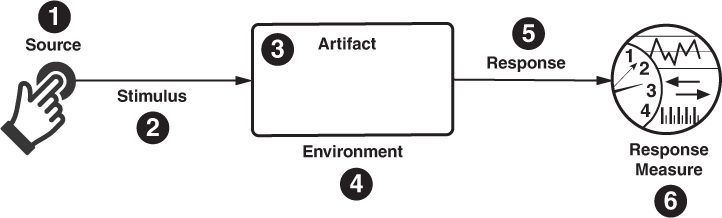
\includegraphics{Figures/qualityattributescenario.jpg}}
\caption{\label{Figure::The parts of a quality attribute scenario} The parts of a quality attribute scenario.}
\end{figure}
\index{Non-functional requirements}\index{testable}\index{unambiguous}\index{Source of stimulus}\index{Stimulus}\index{Environment}\index{Response}\index{Response measure}\index{uptime}\index{error rate}\index{Scenario}
\section{List of Significant Quality Attribute Scenarios\label{Section::SignificantQAS}}
\subsection{Availability\label{subSection::AvailabilityQA}}
\begin{enumerate}
    \item Source of stimulus: A user requests to stitch two images together.
    \item Stimulus: The user clicks on a button to start the stitching process.
    \item Artifact: The two images that the user wants to stitch together.
    \item Environment: The OpenCV Image Stitcher module is running on a computer.
    \item Response: The Image Stitcher module stitches the two images together and displays the result.
    \item Response measure:
    \begin{itemize}
        \item The response measure is the time it takes to stitch the two images together.
        \item The percentage of time that the library is able to process requests and return results without any errors or downtime.
        \item This can be measured using metrics such as uptime, response time, and error rate.
    \end{itemize}
\end{enumerate}
\begin{figure}[H]
\centering
\scalebox{0.6}{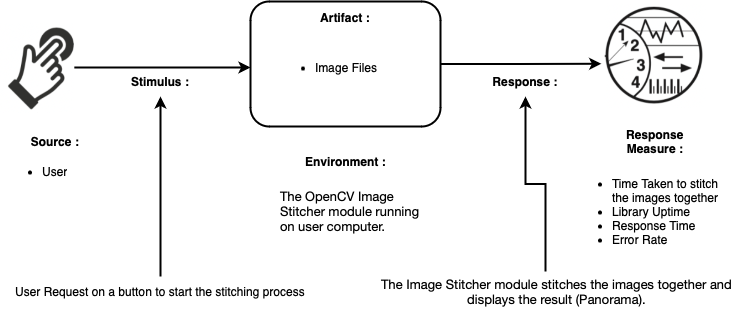
\includegraphics{Figures/Availability.png}}
\caption{\label{Figure::Quality Attribute Scenario for Availability} Quality Attribute Scenario for Availability \cite{drawio}.}
\end{figure}
A high availability score indicates that OpenCV is able to handle a large volume of requests and provide reliable results to users, ensuring that the application is always available and responsive.
In this scenario, the availability quality attribute is met if the Image Stitcher module is able to stitch the two images together in a timely manner. If the Image Stitcher module is not able to stitch the images together, or if it takes a long time to do so, then the availability quality attribute is not met.
\subsection{Deployability\label{subSection::DeployabilityQA}}
\begin{enumerate}
    \item Source of stimulus: A software developer wants to deploy the OpenCV Image Stitcher module in a new application.
    \item Stimulus: The developer downloads the OpenCV Image Stitcher module from the OpenCV website.
    \item Artifact: The OpenCV Image Stitcher module is a C++ library.
    \item Environment: The developer's development environment must have a C++ compiler and the OpenCV libraries installed.
    \item Response: The developer compiles the OpenCV Image Stitcher module and links it to their application.
    \item Response measure: The response measure is the time it takes to deploy the OpenCV Image Stitcher module in the new application.
\end{enumerate} 
\index{Deployability}\index{Energy Efficiency}\index{Integrability}\index{Modifiability}\index{Performance}
\begin{figure}[H]
\centering
\scalebox{0.6}{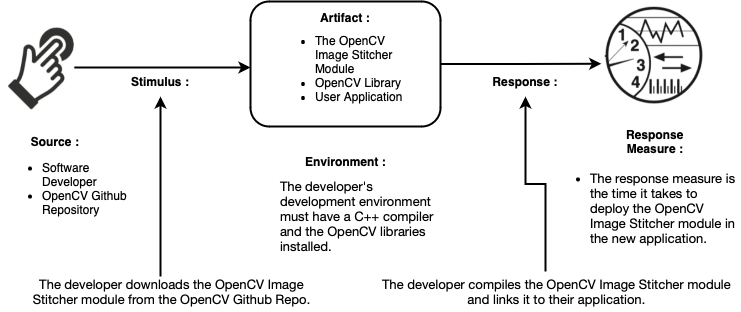
\includegraphics{Figures/Deployability.png}}
\caption{\label{Figure::Quality Attribute Scenario for Deployability} Quality Attribute Scenario for Deployability.}
\end{figure}
In this scenario, the deployability quality attribute is met if the OpenCV Image Stitcher module can be deployed in the new application in a timely manner. If the OpenCV Image Stitcher module cannot be deployed, or if it takes a long time to do so, then the deployability quality attribute is not met.
\subsection{Energy Efficiency\label{subSection::EnergyEfficiencyQA}}
\begin{enumerate}
    \item Source of stimulus: A user wants to use the OpenCV Image Stitcher module to stitch two images together on a mobile device.
    \item Stimulus: The user opens the application that uses the OpenCV Image Stitcher module.
    \item Artifact: The two images that the user wants to stitch together.
    \item Environment: The mobile device has a limited battery life.
    \item Response: The OpenCV Image Stitcher module stitches the two images together and displays the result.
    \item Response measure: The response measure is the amount of energy consumed by the mobile device while the OpenCV Image Stitcher module is running.
\end{enumerate}
\begin{figure}[H]
\centering
\scalebox{0.6}{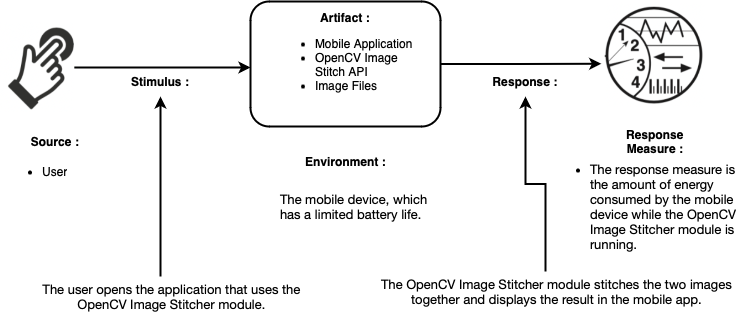
\includegraphics{Figures/energyefficiency.png}}
\caption{\label{Figure::Quality Attribute Scenario for Energy Efficiency} Quality Attribute Scenario for Energy Efficiency.}
\end{figure}
In this scenario, the energy efficiency quality attribute is met if the OpenCV Image Stitcher module is able to stitch the two images together while consuming as little energy as possible. If the OpenCV Image Stitcher module consumes a lot of energy, then the battery life of the mobile device will be reduced.
\subsection{Integrability\label{subSection::IntegrabilityQA}}
\begin{enumerate}
    \item Source of stimulus: Development team
    \item Stimulus: The development team needs to integrate openCV with a new software component.
    \item Artifact: openCV software package, new component
    \item Environment: Development environment with the new software component and its associated hardware and software.
    \item Response: The openCV software package is successfully integrated with the new software component and is fully functional.
    \item Response Measure: The development team measures the time it takes to integrate openCV with the new software component, the number of errors encountered during integration, and the ease of using openCV with the new software component.
\end{enumerate}
\begin{figure}[H]
\centering
\scalebox{0.5}{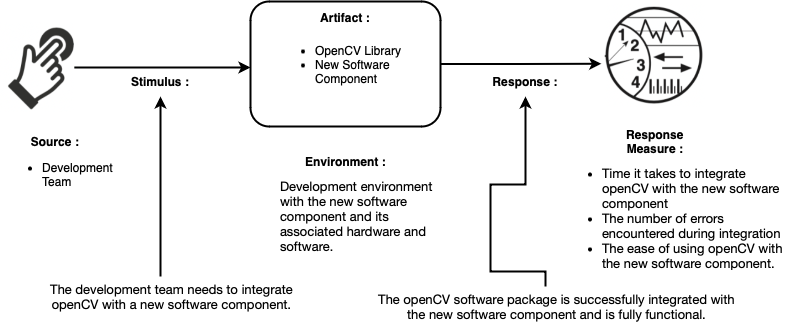
\includegraphics{Figures/Integratability.png}}
\caption{\label{Figure::Quality Attribute Scenario for Integrability} Quality Attribute Scenario for Integrability.}
\end{figure}
Additionally, the team may also measure the impact of the integration on the performance of the new software component and the overall system. The goal is to minimize integration time, errors, and impact on performance, while maximizing ease of use and compatibility with the new software component.
\subsection{Modifiability\label{subSection::ModifiabilityQA}}
\begin{enumerate}
    \item Source of stimulus: Product owner
    \item Stimulus: The product owner requests a new feature to be added to openCV.
    \item Artifact: openCV software package, new feature
    \item Environment: Development environment with the necessary hardware and software.
    \item Response: The development team modifies the openCV software package to include the new feature and ensures that it is fully functional.
    \item Response measure: The development team measures the time it takes to modify openCV to include the new feature, the number of errors encountered during modification, and the impact of the modification on the performance of openCV.
\end{enumerate}
\begin{figure}[H]
\centering
\scalebox{0.5}{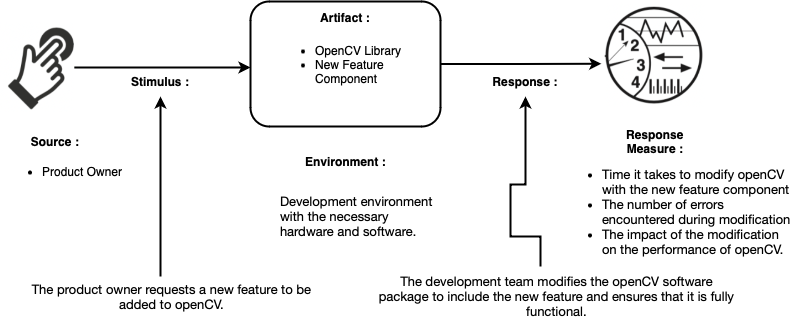
\includegraphics{Figures/modifiability.png}}
\caption{\label{Figure::Quality Attribute Scenario for Modifiability} Quality Attribute Scenario for Modifiability.}
\end{figure}
Additionally, the team may also measure the ease of maintaining the modified code and the impact of the modification on the overall system. The goal is to minimize modification time, errors, and impact on performance, while maximizing ease of maintenance and compatibility with the overall system.
\subsection{Performance\label{subSection::PerformanceQA}}
\begin{enumerate}
    \item Source of stimulus: User
    \item Stimulus: The user requests openCV to process a large image dataset.
    \item Artifact: openCV software package, image dataset, image library
    \item Environment: Production environment with the necessary hardware and software.
    \item Response: openCV processes the large image dataset within an acceptable time frame and with minimal errors.
    \item Response measure: The user measures the time it takes for openCV to process the large image dataset, the number of errors encountered during processing, and the resource utilization of the system during processing.
\end{enumerate}
\begin{figure}[H]
\centering
\scalebox{0.6}{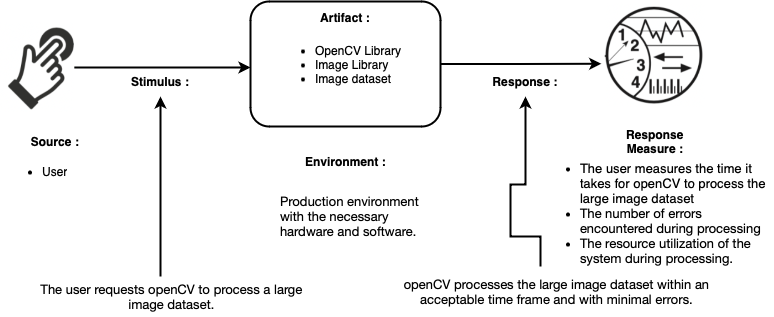
\includegraphics{Figures/Performance.png}}
\caption{\label{Figure::Quality Attribute Scenario for Performance} Quality Attribute Scenario for Performance.}
\end{figure}
Additionally, the user may also measure the accuracy of the processing results and the ease of integrating openCV with other software components in the production environment. The goal is to minimize processing time, errors, and resource utilization, while maximizing accuracy and ease of integration with other software components.
\subsection{Safety\label{subSection::SafetyQA}}
\begin{enumerate}
    \item Source of stimulus: Self-driving car system.
    \item Stimulus: The self-driving car system requests openCV to detect objects on the road and make decisions based on the detected objects.
    \item Artifact: openCV software package, car camera.
    \item Environment: Production environment in a self-driving car with the necessary hardware and software.
    \item Response: openCV accurately detects objects on the road and provides the self-driving car system with the necessary information to make safe driving decisions.
    \item Response measure: The self-driving car system measures the accuracy of openCV's object detection on the road, the number of false positives or false negatives encountered, and the impact of openCV's operation on the safety of the passengers and other vehicles on the road.
\end{enumerate}
\index{Safety}\index{Security}\index{Testability}\index{Usability}
\begin{figure}[H]
\centering
\scalebox{0.6}{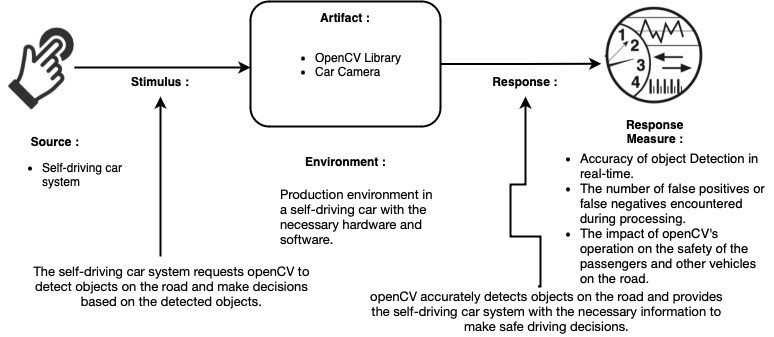
\includegraphics{Figures/Safety.png}}
\caption{\label{Figure::Quality Attribute Scenario for Safety} Quality Attribute Scenario for Safety.}
\end{figure}
Additionally, the system may also measure the ease of integrating openCV with other safety systems in the self-driving car. The goal is to maximize the accuracy of object detection while minimizing any safety hazards or risks associated with openCV's operation in the self-driving car.
\subsection{Security\label{subSection::SecurityQA}}
\begin{enumerate}
    \item Source of stimulus: Unauthorized user
    \item Stimulus: The unauthorized user attempts to gain access to sensitive information or disrupt the operation of openCV.
    \item Artifact: openCV software package, Security log report
    \item Environment: Production environment with the necessary hardware and software.
    \item Response: openCV detects and prevents the unauthorized user's attempts to gain access to sensitive information or disrupt the system's operation and does not compromise the security of the system or any sensitive information.
    \item Response measure: The system measures the number of successful and unsuccessful attempts by the unauthorized user to gain access to sensitive information or disrupt the system's operation, the impact of the unauthorized user's attempts on the security of the system and any sensitive information, and the effectiveness of openCV's security measures in preventing the unauthorized user's attempts.
\end{enumerate}
\begin{figure}[H]
\centering
\scalebox{0.5}{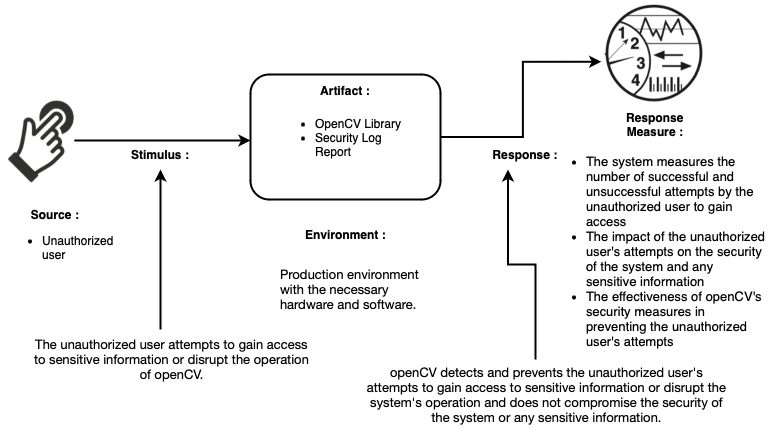
\includegraphics{Figures/Security.png}}
\caption{\label{Figure::Quality Attribute Scenario for Security} Quality Attribute Scenario for Security.}
\end{figure}
Additionally, the system may also measure the ease of maintaining and updating openCV's security measures to address any new vulnerabilities or threats. The goal is to minimize the number of successful unauthorized access attempts and their impact on the security of the system and any sensitive information.
\subsection{Testability\label{subSection::TestabilityQA}}
\begin{enumerate}
    \item Source of stimulus: Testing team
    \item Stimulus: The testing team needs to test the accuracy and performance of the openCV Image Stitching module in a real-world scenario.
    \item Artifact: openCV Image Stitching module, Image files
    \item Environment: Real-world environment with the necessary hardware and software on tester's computer.
    \item Response: The openCV Image Stitching module accurately stitches images in the real-world scenario and performs within acceptable performance parameters.
    \item Response measure: The testing team measures the accuracy of the openCV Image Stitching module in stitching images in the real-world scenario, the number of errors encountered during stitching, and the performance of the module in terms of processing time and resource utilization. Test-cases pass percentage for unique scenarios. Test Coverage percentage of openCV Image Stitching module.
\end{enumerate}
\begin{figure}[H]
\centering
\scalebox{0.5}{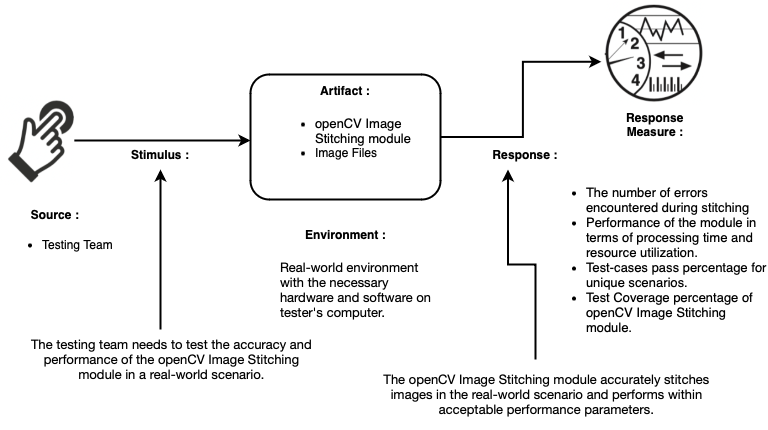
\includegraphics{Figures/Testability.png}}
\caption{\label{Figure::Quality Attribute Scenario for Testability} Quality Attribute Scenario for Testability.}
\end{figure}
Additionally, the team may also measure the ease of testing the openCV Image Stitching module in the real-world scenario and the effectiveness of any testing tools or frameworks used. The goal is to maximize the accuracy and performance of the openCV Image Stitching module in the real-world scenario while minimizing any testing time and effort required.
\subsection{Usability\label{subSection::UsabilityQA}}
\begin{enumerate}
    \item Source of stimulus: User
    \item Stimulus: The user needs to use openCV to perform image processing tasks.
    \item Artifact: openCV software package, image files
    \item Environment: User's environment with the necessary hardware and software.
    \item Response: The user is able to use openCV to perform image processing tasks with ease and efficiency.
    \item Response measure: The user measures the ease of learning and using openCV to perform image processing tasks, the time it takes to complete the tasks, and the user satisfaction with the user interface and overall usability of openCV.
\end{enumerate}
\begin{figure}[H]
\scalebox{0.5}{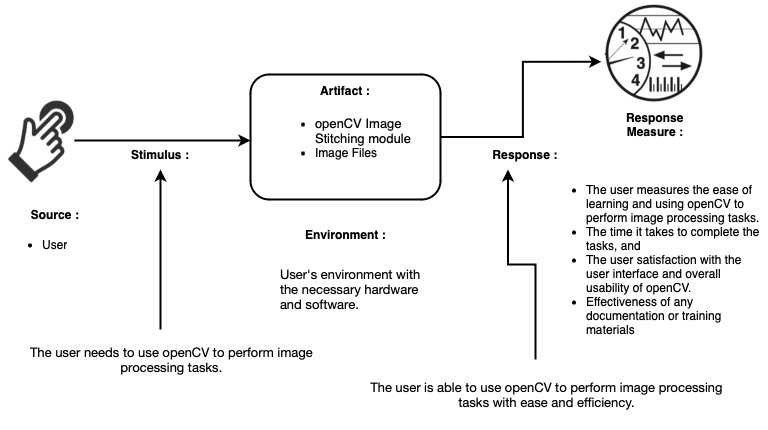
\includegraphics{Figures/Usability.png}}
\caption{\label{Figure::Quality Attribute Scenario for Usability} Quality Attribute Scenario for Usability.}
\end{figure}
Additionally, the user may also measure the effectiveness of any documentation or training materials provided with openCV. The goal is to maximize the ease of use and efficiency of openCV for image processing tasks, while minimizing the time and effort required to learn and use the software.
\section{Evaluation of Business risk and Architectural Significance\label{Section::QAratings}}
\begin{longtable}{|l|c|c|}
\hline
\textbf{Quality Attribute} & \textbf{Business Value (a)} & \textbf{Effect on Architecture (b)} \\
\hline
Availability & H & M \\
Deployability & M & M \\
Energy Efficiency & L & M \\
Integrability & M & M \\
Modifiability & H & M \\
Performance & H & H \\
Safety & H & H \\
Security & H & H \\
Testability & H & M \\
Usability & M & M \\
\hline
\caption{Quality Attribute Evaluation \label{Table::Quality Attribute Evaluation}}
\end{longtable}
\newpage
\subsection{Understanding the values}
Grading Scale Used:\newline
\newline
\underline{\textbf{Rating:}} (a, b):\newline
\textbf{a:} the ASR’s\index{ASR!Architecturally significant requirement} business value\index{Business Value}(importance)\newline
\textbf{b:} the effect on the architecture(difficulty)\newline
\\
\underline{\textbf{Key:}}\newline
\textbf{H}=high\newline
\textbf{M}=medium\newline
\textbf{L}=low\newline
\begin{enumerate}
    \item Availability: openCV is a mature library with a large community of users and developers. There are many different ways to install and use openCV, which makes it easy to deploy in a variety of environments. This is why we rated availability as high.
    \item Deployability: openCV is available for a variety of platforms, including Windows, Linux, and macOS. There are also many different ways to deploy openCV, such as as a static library, a shared library, or a Docker image. This is why we rated deployability as medium.
    \item Energy Efficiency: openCV uses a variety of techniques to optimize its performance, such as using hardware acceleration and image compression. This is why we rated energy efficiency as low.
    \item Integrability: openCV provides a variety of APIs, such as C++, Python, and Java, which make it easy to integrate with other languages and frameworks. This is why we rated integrabilty as medium.
    \item Modifiability: openCV is a open source library, which means that the source code is available for anyone to modify. This makes it easy to customize openCV to meet the specific needs of a project. This is why we rated modifiability as high.
    \item Performance: openCV is designed to be fast and efficient, even on resource-constrained devices. This is why we rated performance as high.
    \item Safety: openCV is designed to be secure and reliable, even in critical applications. This is why I rated safety as high.
    \item Security: openCV is designed to be resistant to attack and intrusion. This is why we rated security as high.
    \item Testability: openCV provides a variety of tools and resources to help developers test their code. This makes it easy to ensure that openCV is working properly before it is deployed in production. This is why we rated testability as high.
    \item Usability: openCV provides a variety of documentation and tutorials to help developers get started. This makes it easy for anyone to use openCV, regardless of their experience level. This is why we rated usability as medium.
\end{enumerate}
\section{Utiltity Tree\label{Section::utilityTree}}
\subsection{Introduction}
\paragraph{} A utility tree starts with the root node "Utility" representing the overall "goodness" of the system. Major Quality Attributes (QAs) are listed under the root node. Each QA is then further refined with specific aspects relevant to the system. These refinements can be broken down into specific Quality Attribute Scenarios (ASRs).
\paragraph{} ASRs are placed as leaves on the tree and evaluated based on business value and technical risk. Business value is assessed as high, medium, or low, indicating the importance of meeting the requirement. Technical risk is evaluated as high, medium, or low, reflecting the level of concern and confidence in meeting the ASR.
\paragraph{} In summary, a utility tree outlines the system's QAs, their refinements, and ASRs as scenarios. These scenarios are then evaluated based on business value and technical risk.
\subsection{Tabular form of Utility Tree}
\begin{figure}[H]
\centering
\scalebox{0.55}{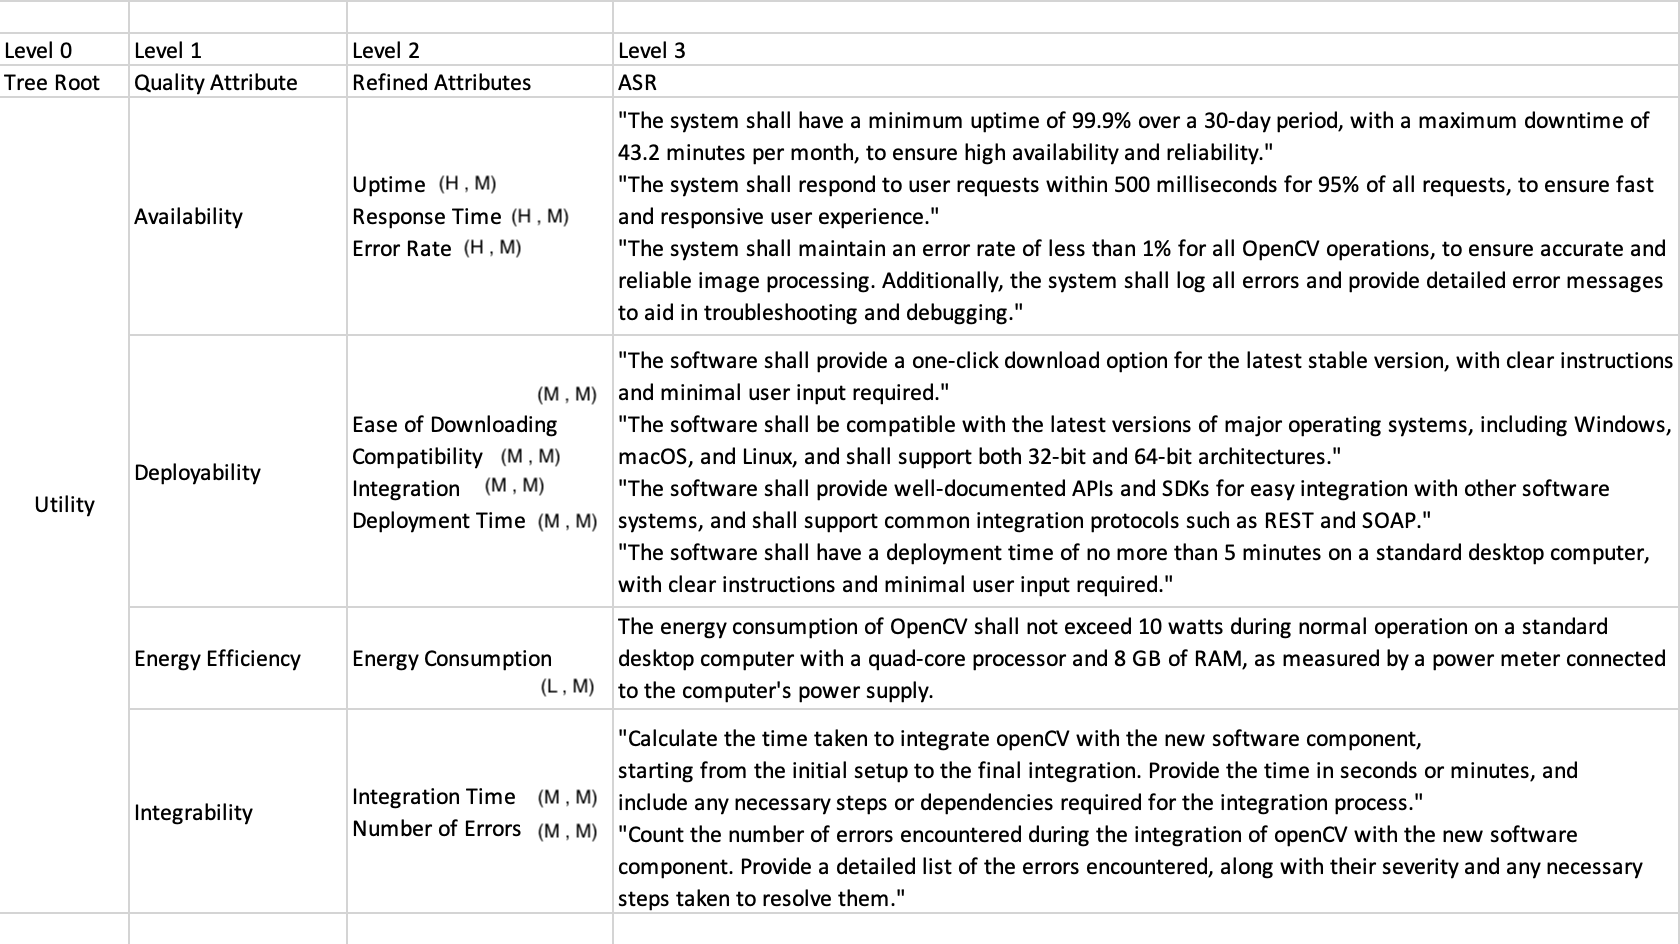
\includegraphics{Figures/UtilityTree1.png}}
\caption{\label{Figure::UtilityTree1} Utility Tree - 1.}
\end{figure}
\begin{figure}[H]
\centering
\scalebox{0.5}{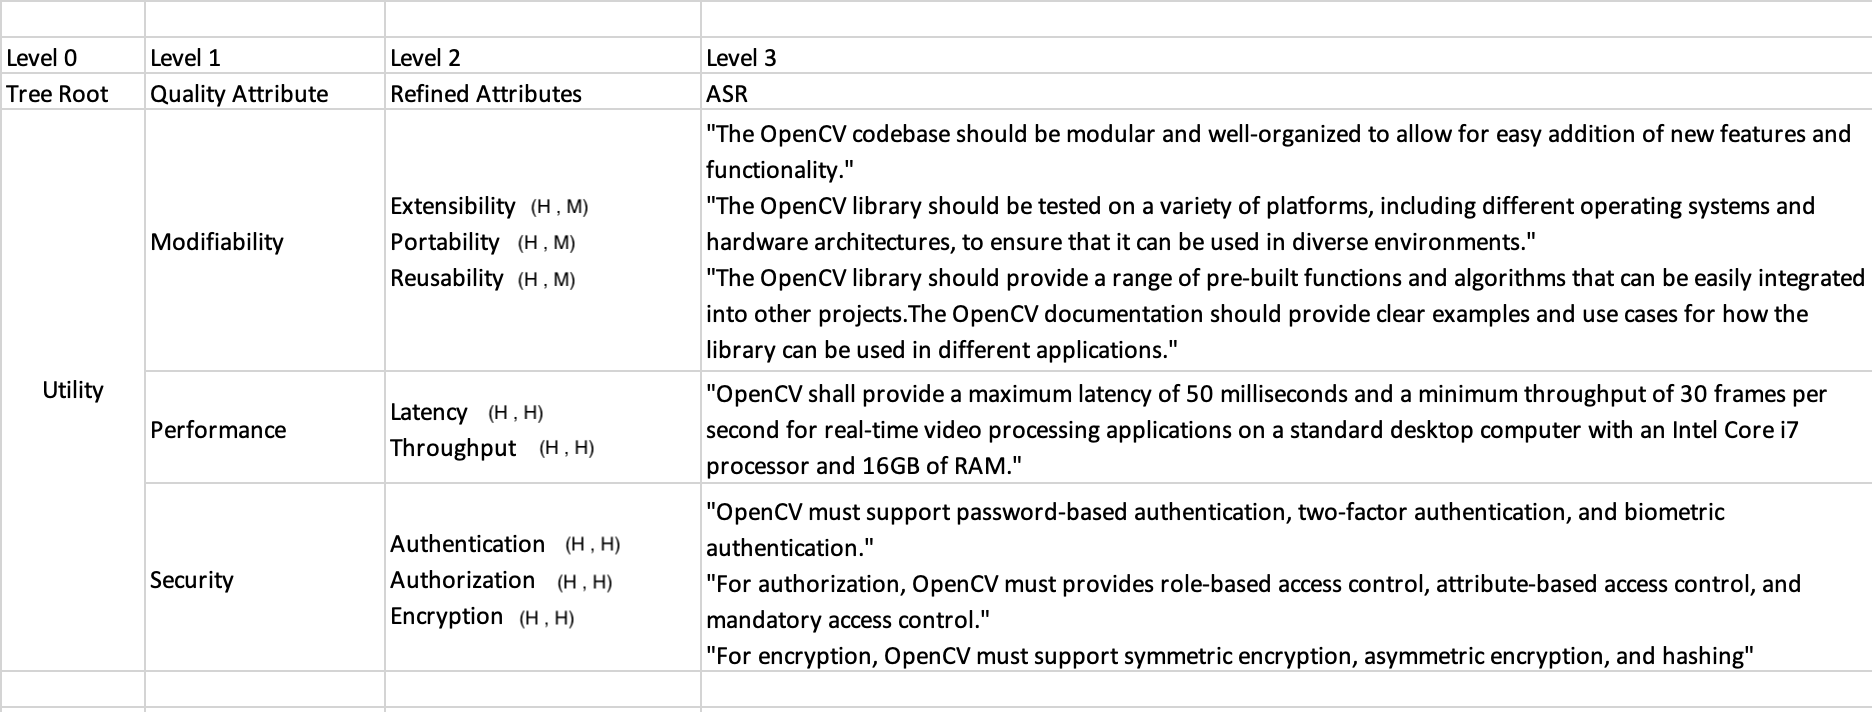
\includegraphics{Figures/UtilityTree2.png}}
\caption{\label{Figure::UtilityTree2} Utility Tree - 2.}
\end{figure}
\begin{figure}[H]
\centering
\scalebox{0.5}{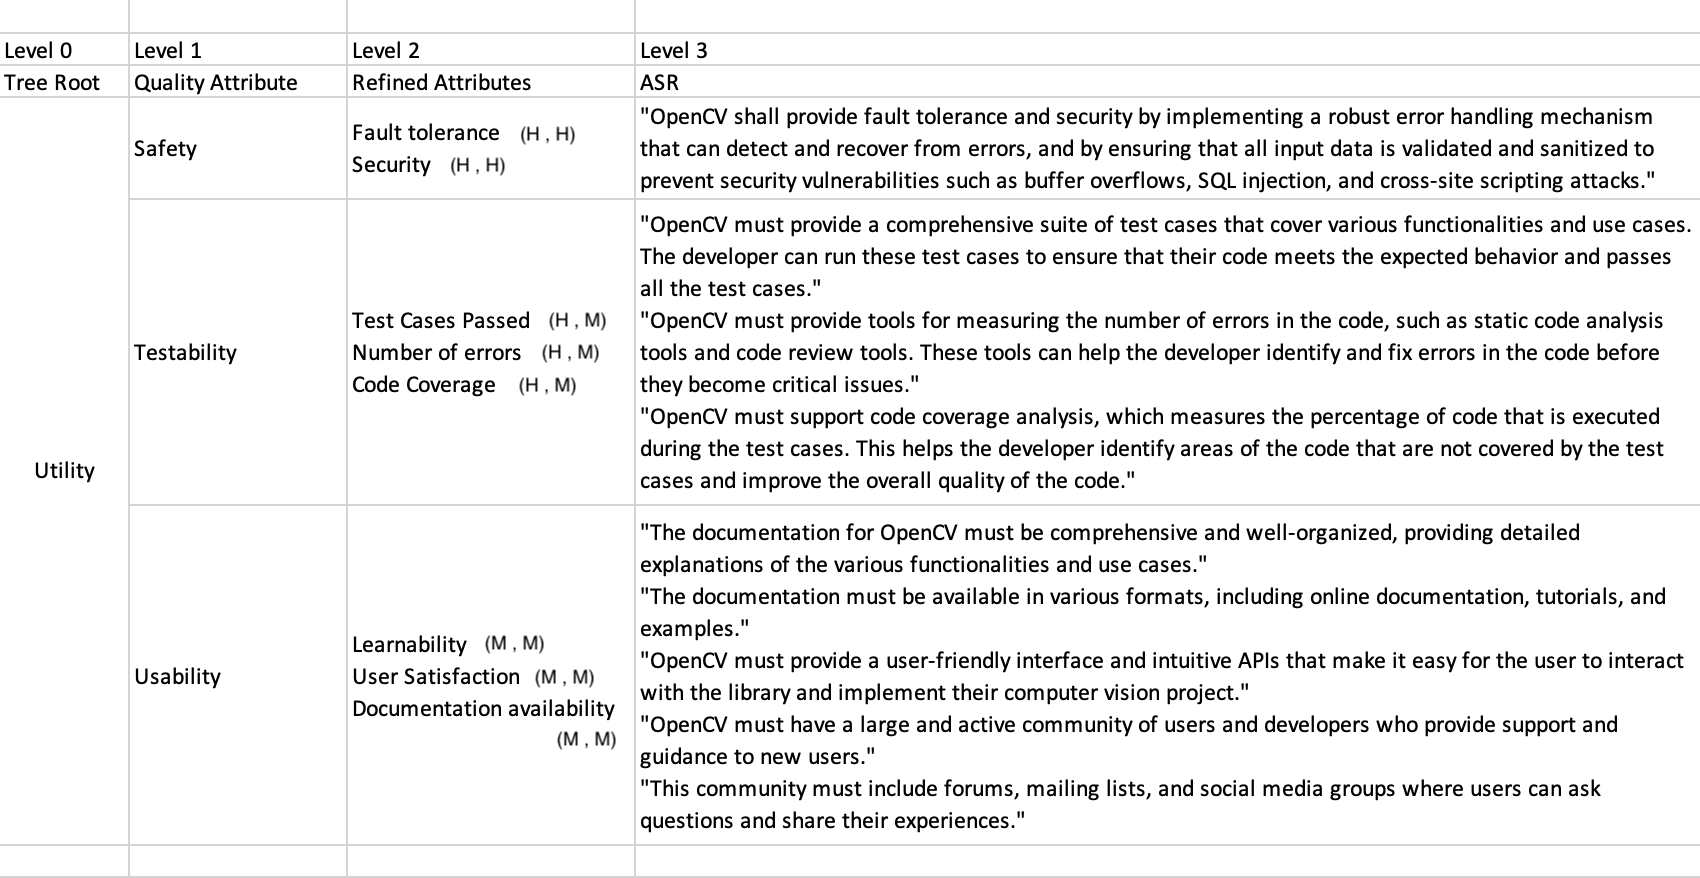
\includegraphics{Figures/UtilityTree3.png}}
\caption{\label{Figure::UtilityTree3} Utility Tree - 3.}
\end{figure}